%% GENERATED by tools/from_docs.py from stepss-docs. Do not edit by hand:
%% edit the page named below in stepss-docs and regenerate.
%% source: stepss-docs/src/content/docs/models/custom-governors.mdx

\chapter{Other turbine-governor models}\label{doc:model-tor-custom}

This page documents the custom turbine-governor (\texttt{tor\_}) models in RAMSES. These models are implemented in Fortran using the legacy multi-subroutine API and cover a wide range of prime-mover types: thermal (steam), gas turbine, hydraulic, nuclear, and simplified equivalents.

\begin{docsnote}{Usage in Dynamic Data Files}

Governor/torque models in RAMSES are defined as sub-records within a \texttt{SYNC\_MACH} block using the \texttt{TOR} keyword, followed by the model name and its parameters. They are not standalone records. The \texttt{TOR} line appears after the \texttt{EXC} (exciter) line, and the \texttt{;} at the end closes the entire \texttt{SYNC\_MACH} block.

\begin{Verbatim}
SYNC_MACH name bus FP FQ P Q SNOM Pnom H D IBRATIO
                    XT  Xl  Xd  X'd  X"d  Xq  X'q  X"q  m  n  Ra  T'do  T"do  T'qo  T"qo
              EXC model_name  param1  param2  ...
              TOR model_name  param1  param2  ... ;
\end{Verbatim}

This page documents the four governors built into every RAMSES distribution, \texttt{CONSTANT}, \texttt{1ST\_ORDER}, \texttt{HYDRO\_GENERIC1} and \texttt{THERMAL\_GENERIC1}, which take no prefix and are written in uppercase, together with \texttt{HYDRO\_DG}, registered since 3.76.

It also documents \texttt{GASTURBM}, \texttt{GOVCLASM}, \texttt{GOVHYDR} and \texttt{GOVNUC}, which the family dispatcher has handled directly since 3.79. Before 3.79 they were compiled under no name and RAMSES rejected them in a data file.

The IEEE governors, \texttt{DEGOV1}, \texttt{ENTSOE\_simp}, \texttt{GAST}, \texttt{TGOV1} and \texttt{HYGOV}, are on the \hyperref[doc:model-tor-ieee]{IEEE Governors} page. For the whole catalogue at a glance, see the \hyperref[doc:model-index]{Model Reference index}.

\end{docsnote}

\begin{center}\rule{0.5\linewidth}{0.5pt}\end{center}

\section{\texorpdfstring{CONSTANT (\texttt{tor\_constant})}{CONSTANT (tor\_constant)}}\label{model-tor-custom:constant-tor_constant}

The data-file model name is \texttt{CONSTANT}.

\subsection{Scientific Description}\label{model-tor-custom:scientific-description}

The \texttt{tor\_constant} model provides a \textbf{constant mechanical torque} source. The mechanical torque is fixed at its initialisation value and does not respond to speed deviations or load changes:

\[
T_m(t) = T_{m0} \quad \forall t
\]

The single algebraic state satisfies:

\[
f(1) = x(1) - T_{m0} = 0
\]

The observable output is mechanical power:

\[
P_m = T_m \cdot \omega
\]

\textbf{Implementation details:}
- \texttt{nbxvar\ =\ 1}, \texttt{nbzvar\ =\ 0}, \texttt{nbdata\ =\ 0}
- One additional parameter: \texttt{prm(1)\ =\ Tm0} (set at initialisation from load-flow)
- Observable: \texttt{Pm\ =\ x(1)\ *\ omega}

\subsection{Parameters}\label{model-tor-custom:parameters}

\begin{small}\begin{longtable}[]{@{}
  >{\raggedright\arraybackslash}p{(\linewidth - 4\tabcolsep) * \real{0.2899}}
  >{\raggedright\arraybackslash}p{(\linewidth - 4\tabcolsep) * \real{0.7101}}
@{}}
\toprule\noalign{}
\begin{minipage}[b]{\linewidth}\raggedright
Parameter
\end{minipage} & \begin{minipage}[b]{\linewidth}\raggedright
Description
\end{minipage} \\
\midrule\noalign{}
\endhead
\bottomrule\noalign{}
\endlastfoot
\emph{(none)} & No user-supplied parameters. \(T_{m0}\) is taken from the load-flow initialisation. \\
\end{longtable}\end{small}

\subsection{Usage Example}\label{model-tor-custom:usage-example}

\textbf{RAMSES Data File}

\begin{Verbatim}
SYNC_MACH g6  g6  1. 1.  0.  0.   400. 360. 6. 0. 2.05
                    XT   0.15  2.2  0.3    0.2   2.   0.4  0.2  0.1  6.0257  0.  7.00  0.05  1.5  0.05
              EXC GENERIC1   3.0618 -0.1  1.  0.  100. -1. -20.0  10.  120. 5.  12.5 0.1  0.  5.
                                1     75.   15.    0.22    0.012     0.22    0.012    -0.1    0.1
              TOR CONSTANT ;
\end{Verbatim}

\textbf{Notes}

\begin{itemize}
\tightlist
\item
  Useful for machines operating at fixed setpoint, for testing generator models in isolation, or as a placeholder.
\item
  The mechanical power observable \(P_m = T_m \cdot \omega\) will vary slightly with speed changes.
\item
  \texttt{TOR\ CONSTANT} takes no parameters, \(T_{m0}\) is set automatically from the load-flow initialisation.
\end{itemize}

\begin{center}\rule{0.5\linewidth}{0.5pt}\end{center}

\section{\texorpdfstring{1ST\_ORDER (\texttt{tor\_1storder})}{1ST\_ORDER (tor\_1storder)}}\label{model-tor-custom:st_order-tor_1storder}

The data-file model name is \texttt{1ST\_ORDER} (uppercase, with the underscore).

\subsection{Scientific Description}\label{model-tor-custom:scientific-description-1}

The \texttt{tor\_1storder} model is a \textbf{first-order speed governor} with droop and a two-mass (HP/LP) turbine representation. It captures the primary frequency response through a proportional-droop speed controller with a first-order lag.

\textbf{Speed controller with droop \(R\):}

The mechanical torque setpoint is:

\[
T_{set} = T_{m0} - \frac{\omega - 1}{R}
\]

The HP torque tracks \(T_{set}\) through a first-order lag with time constant \(T_2\):

\[
\frac{d x_1}{dt} = \frac{1}{T_2}\left(T_{set} - x_1\right)
\]

The LP (shaft) torque is a weighted combination:

\[
x_2 = (1 - F_{HP}) \cdot x_1 + F_{HP} \cdot T_{set}
\]

where \(F_{HP}\) is the fraction of power generated in the HP stage.

From the Fortran equations:

\begin{Verbatim}
f(1) = (-x(1) + (prm(4) - (omega-1.d0)/prm(3))) / prm(2)
f(2) = (1.d0-prm(1))*x(1) + prm(1)*(prm(4)-(omega-1.d0)/prm(3)) - x(2)
\end{Verbatim}

i.e.:
- \texttt{prm(1)\ =\ FHP} (HP fraction), \texttt{prm(2)\ =\ T2} (time constant), \texttt{prm(3)\ =\ R} (droop)
- \texttt{prm(4)\ =\ Tm0} (setpoint, set at init)

\textbf{Implementation details:}
- \texttt{nbxvar\ =\ 2}, \texttt{nbzvar\ =\ 0}, \texttt{nbdata\ =\ 3}
- State 1 = HP torque \texttt{x(1)}, State 2 = LP torque \texttt{x(2)}
- Observables: \texttt{HP\ torque}, \texttt{LP\ torque}

\begin{figure}[htbp]
\centering
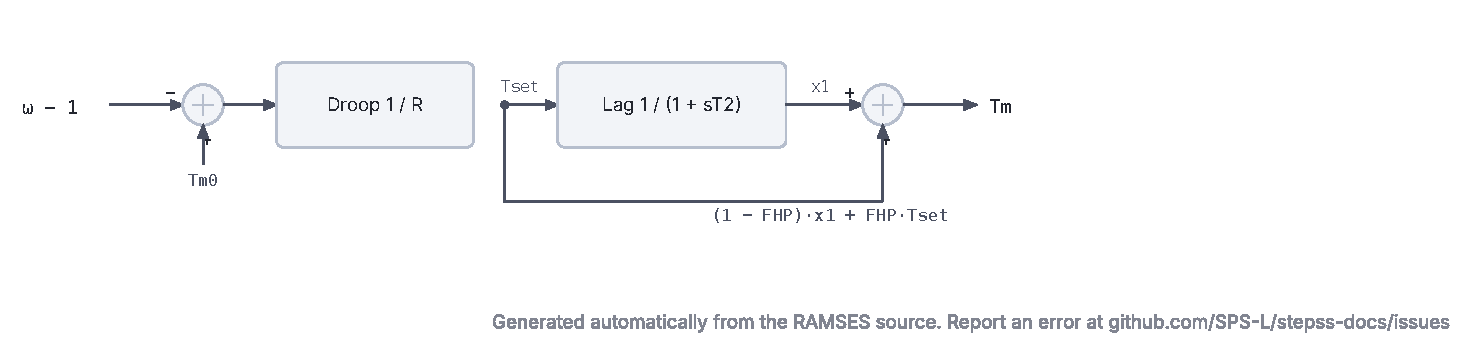
\includegraphics[width=0.98\linewidth]{figures/tor-1storder-light}
\caption{1ST\_ORDER governor block diagram.}
\end{figure}

\subsection{Parameters}\label{model-tor-custom:parameters-1}

\begin{small}\begin{longtable}[]{@{}ll@{}}
\toprule\noalign{}
Parameter & Description \\
\midrule\noalign{}
\endhead
\bottomrule\noalign{}
\endlastfoot
\texttt{FHP} & Fraction of torque produced by the HP turbine stage (0--1) \\
\texttt{T2} & Governor/HP turbine time constant (s) \\
\texttt{R} & Speed droop (pu/pu) \\
\end{longtable}\end{small}

\subsection{Usage Example}\label{model-tor-custom:usage-example-1}

\textbf{RAMSES Data File}

\begin{Verbatim}
SYNC_MACH g1  g1  1. 1.  0.  0.   800. 760. 3. 0. 0.95
                    XT   0.15  1.1  0.25   0.2   0.7   *   0.2  0.1  6.0257  0.  5.00  0.05  *  0.1
              EXC GENERIC1   1.8991 -0.1  0.  1.  100. -1. -11  10.  70.  10.  20. 0.1  0.  4.
                                1     75.   15.    0.2    0.01     0.2    0.01    -0.1    0.1
              TOR 1ST_ORDER  0.30  0.50  0.05 ;  ! FHP  T2  R
\end{Verbatim}

\textbf{Notes}

\begin{itemize}
\tightlist
\item
  \texttt{FHP\ =\ 0} makes the model a pure first-order lag on the total torque.
\item
  \texttt{FHP\ =\ 1} bypasses the HP lag entirely; the torque instantly tracks the droop setpoint.
\item
  Typical primary-frequency response studies use \texttt{R\ =\ 0.04}--\texttt{0.05}.
\end{itemize}

\begin{center}\rule{0.5\linewidth}{0.5pt}\end{center}

\section{\texorpdfstring{THERMAL\_GENERIC1 (\texttt{tor\_thermal\_generic1})}{THERMAL\_GENERIC1 (tor\_thermal\_generic1)}}\label{model-tor-custom:thermal_generic1-tor_thermal_generic1}

The data-file model name is \texttt{THERMAL\_GENERIC1}.

\subsection{Scientific Description}\label{model-tor-custom:scientific-description-2}

The \texttt{tor\_thermal\_generic1} model is a \textbf{generic multi-stage steam turbine governor}, suitable for both single-shaft and cross-compound units. It includes a speed controller with rate-limiting, a three-section steam chest/reheater, and separate HP, MP, and LP turbine stages.

\begin{figure}[htbp]
\centering
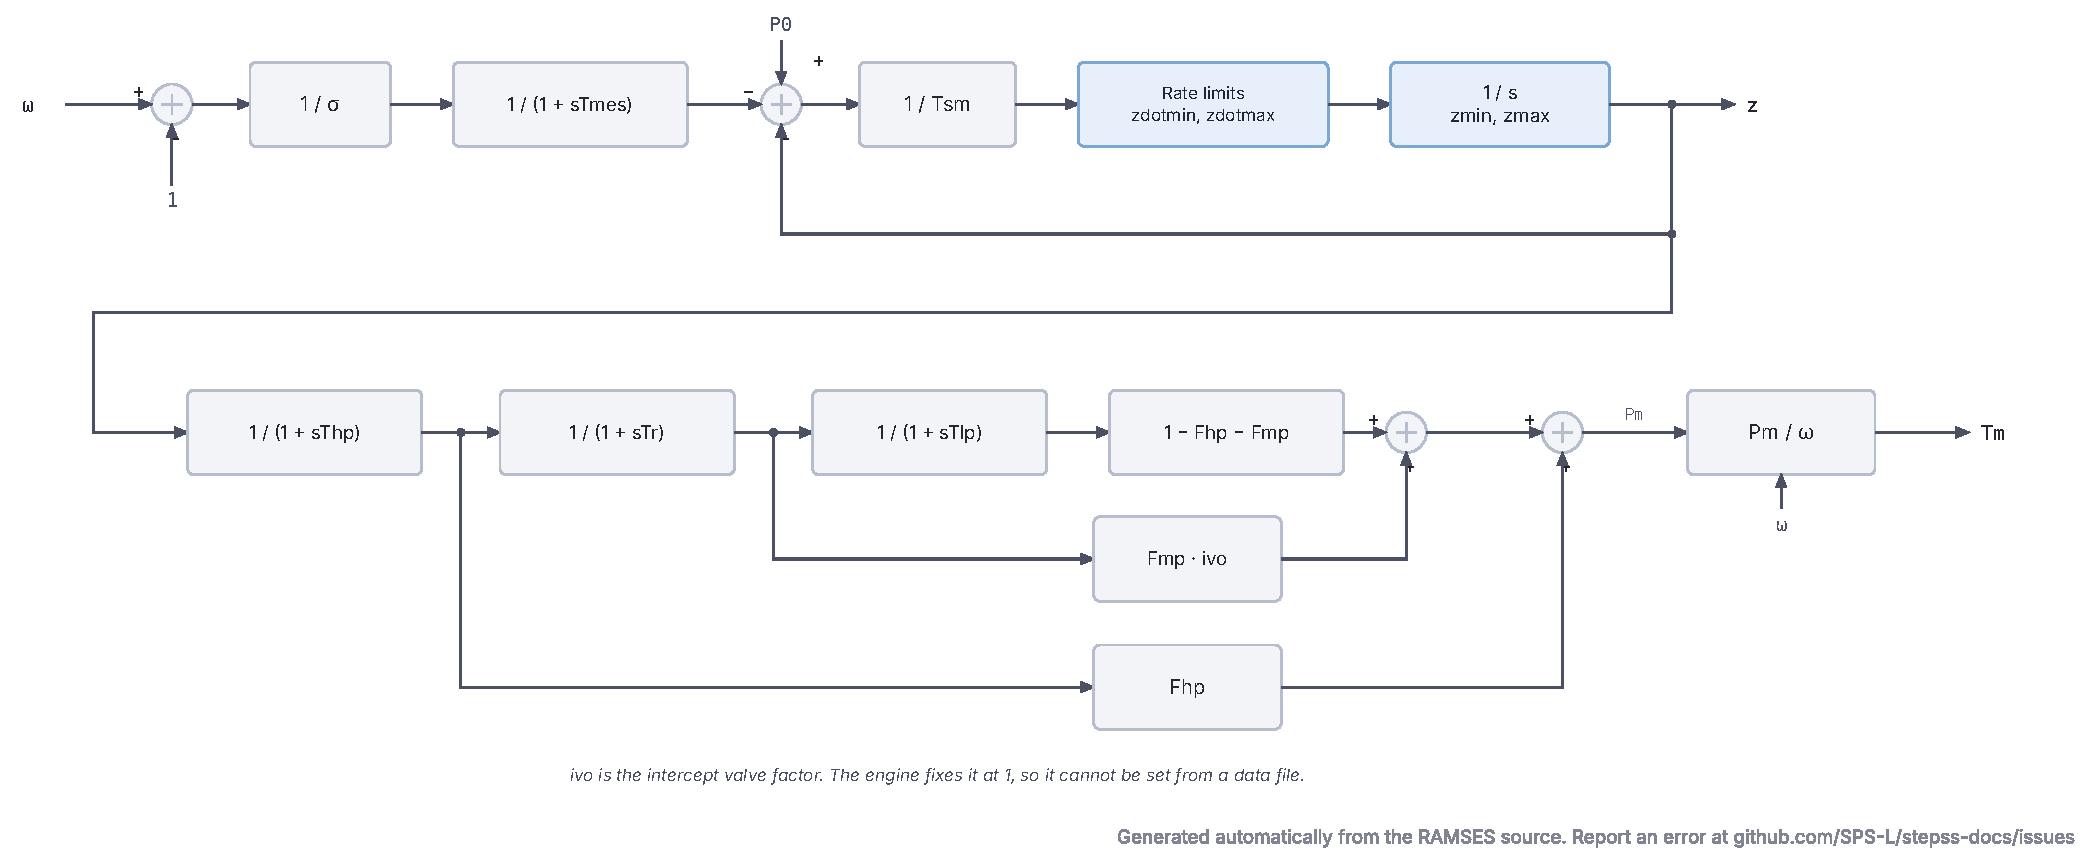
\includegraphics[width=0.98\linewidth]{figures/tor-thermal-generic1-light}
\caption{THERMAL\_GENERIC1 block diagram.}
\end{figure}

\textbf{Speed governor:}

The speed deviation is divided by the droop \(\sigma\) and measured with time constant \(T_{mes}\):

\[
T_{mes}\,\dot{x}_1 = -x_1 + \frac{\omega - 1}{\sigma}
\]

The gate demand is what remains of the power setpoint after that term and the current gate position are taken off:

\[
e_{gov} = P_0 - x_1 - z
\]

It is divided by the servo time constant \(T_{sm}\), rate-limited to \([zdot_{min},\, zdot_{max}]\), and integrated into the gate opening \(z\) within \([z_{min},\, z_{max}]\).

\textbf{Turbine power stages:}

The gate opening drives three lags in series, the reheat stage carrying the initial valve opening \(ivo\) as a factor:

\[
T_{hp}\,\dot{x}_{hp} = -x_{hp} + z, \qquad
T_r\,\dot{x}_r = -x_r + x_{hp}, \qquad
T_{lp}\,\dot{x}_{lp} = -x_{lp} + ivo\,x_r
\]

Each stage contributes its own fraction of the power, and the three fractions sum to one:

\[
P_{mHP} = F_{hp}\,x_{hp}, \qquad
P_{mMP} = F_{mp}\,ivo\,x_r, \qquad
P_{mLP} = (1 - F_{hp} - F_{mp})\,x_{lp}
\]

Total mechanical power, and the torque delivered to the shaft:

\[
P_m = P_{mHP} + P_{mMP} + P_{mLP}, \qquad T_m = \frac{P_m}{\omega}
\]

\textbf{Parameters:}

\begin{small}\begin{longtable}[]{@{}lll@{}}
\toprule\noalign{}
Parameter & Index & Description \\
\midrule\noalign{}
\endhead
\bottomrule\noalign{}
\endlastfoot
\texttt{sigma} & 1 & Speed droop (pu/pu) \\
\texttt{Tmes} & 2 & Speed measurement time constant (s) \\
\texttt{Tsm} & 3 & Servo/gate time constant (s) \\
\texttt{zdotmin} & 4 & Minimum gate rate (pu/s), also additional parameter \\
\texttt{zdotmax} & 5 & Maximum gate rate (pu/s) \\
\texttt{zmin} & 6 & Minimum gate opening (pu) \\
\texttt{zmax} & 7 & Maximum gate opening (pu) \\
\texttt{Thp} & 8 & HP turbine time constant (s) \\
\texttt{Fhp} & 9 & HP power fraction \\
\texttt{Tr} & 10 & Reheater / MP time constant (s) \\
\texttt{Fmp} & 11 & MP power fraction \\
\texttt{Tlp} & 12 & LP turbine time constant (s) \\
\end{longtable}\end{small}

\textbf{Implementation details:}
- \texttt{nbxvar\ =\ 10}, \texttt{nbzvar\ =\ 2}, \texttt{nbdata\ =\ 12}, \texttt{nbaddpar\ =\ 2}
- Additional: \texttt{prm(13)\ =\ P0} (initial power), \texttt{prm(14)\ =\ ivo} (initial valve opening)
- Observables: \texttt{z}, \texttt{PmHP}, \texttt{PmMP}, \texttt{PmLP}, \texttt{Pm}

\subsection{Usage Example}\label{model-tor-custom:usage-example-2}

\textbf{RAMSES Data File}

\begin{Verbatim}
SYNC_MACH g1  g1  1. 1.  0.  0.   800. 760. 3. 0. 0.95
                    XT   0.15  1.1  0.25   0.2   0.7   *   0.2  0.1  6.0257  0.  5.00  0.05  *  0.1
              EXC GENERIC1   1.8991 -0.1  0.  1.  100. -1. -11  10.  70.  10.  20. 0.1  0.  4.
                                1     75.   15.    0.2    0.01     0.2    0.01    -0.1    0.1
              TOR THERMAL_GENERIC1  0.05  0.02  0.20  -0.10  0.10  0.0  1.05  0.30  0.30  7.0  0.40  0.50 ;
              !                     sigma Tmes  Tsm  zdotmin zdotmax zmin zmax  Thp   Fhp   Tr   Fmp   Tlp
\end{Verbatim}

\textbf{Notes}

\begin{itemize}
\tightlist
\item
  The LP fraction is \texttt{1\ -\ Fhp\ -\ Fmp}; ensure \texttt{Fhp\ +\ Fmp\ \ensuremath{\le}\ 1}.
\item
  Set \texttt{Tmes\ =\ 0} to bypass the speed measurement filter (instantaneous speed sensing).
\item
  Rate limits \texttt{zdotmin}/\texttt{zdotmax} are critical for AGC studies.
\end{itemize}

\begin{center}\rule{0.5\linewidth}{0.5pt}\end{center}

\section{\texorpdfstring{HYDRO\_GENERIC1 (\texttt{tor\_hydro\_generic1})}{HYDRO\_GENERIC1 (tor\_hydro\_generic1)}}\label{model-tor-custom:hydro_generic1-tor_hydro_generic1}

The data-file model name is \texttt{HYDRO\_GENERIC1}.

\subsection{Scientific Description}\label{model-tor-custom:scientific-description-3}

The \texttt{tor\_hydro\_generic1} model is a \textbf{generic hydraulic turbine governor} with a penstock (water column) and PI controller. It implements the standard hydraulic governor structure following IEEE Std 1110 conventions.

\textbf{PI speed governor:}

The speed error with droop \(\sigma\):

\[
e = (P_0 - P_{meas}) \cdot \sigma + (1 - \omega)
\]

A PI controller with gains \(K_P\) and \(K_I\) drives the gate demand:

\[
\dot{x}_{I} = K_I \cdot e
\]

\[
z_{demand} = K_P \cdot e + x_I
\]

The gate is rate-limited by \(LIM_{\dot{z}}\) and position-limited by \([0, 1]\), with a servo time constant \(T_{sm}\).

\textbf{Water column (penstock):}

The flow \(Q\) and head \(H\) are related by the water-starting time \(T_W\):

\[
T_W \cdot \frac{dQ}{dt} = 1 - H
\]

The head is:

\[
H = \left(\frac{Q_{v} + T_m (1 - Q_v)}{z}\right)^2
\]

where \(Q_v\) is the no-load flow fraction.

\textbf{Turbine mechanical torque:}

\[
T_m = \sqrt{H} \cdot (Q - Q_v \cdot \sqrt{H})
\]

\[
P_m = T_m \cdot \omega
\]

\textbf{Parameters:}

\begin{small}\begin{longtable}[]{@{}lll@{}}
\toprule\noalign{}
Parameter & Index & Description \\
\midrule\noalign{}
\endhead
\bottomrule\noalign{}
\endlastfoot
\texttt{SIGMA} & 1 & Speed droop (pu/pu) \\
\texttt{Tmes} & 2 & Speed measurement time constant (s) \\
\texttt{Qv} & 3 & No-load water flow fraction (pu) \\
\texttt{KP} & 4 & PI proportional gain \\
\texttt{KI} & 5 & PI integral gain \\
\texttt{TSM} & 6 & Gate servo time constant (s) \\
\texttt{LIMZDOT} & 7 & Gate velocity limit (pu/s) \\
\texttt{TW} & 8 & Water starting time (s) \\
\end{longtable}\end{small}

\textbf{Implementation details:}
- \texttt{nbxvar\ =\ 6}, \texttt{nbzvar\ =\ 2}, \texttt{nbdata\ =\ 8}, \texttt{nbaddpar\ =\ 1}
- Additional: \texttt{prm(9)\ =\ P0} (initial electrical power)
- Observables: \texttt{z}, \texttt{Q}, \texttt{H}, \texttt{Pm}

\begin{figure}[htbp]
\centering
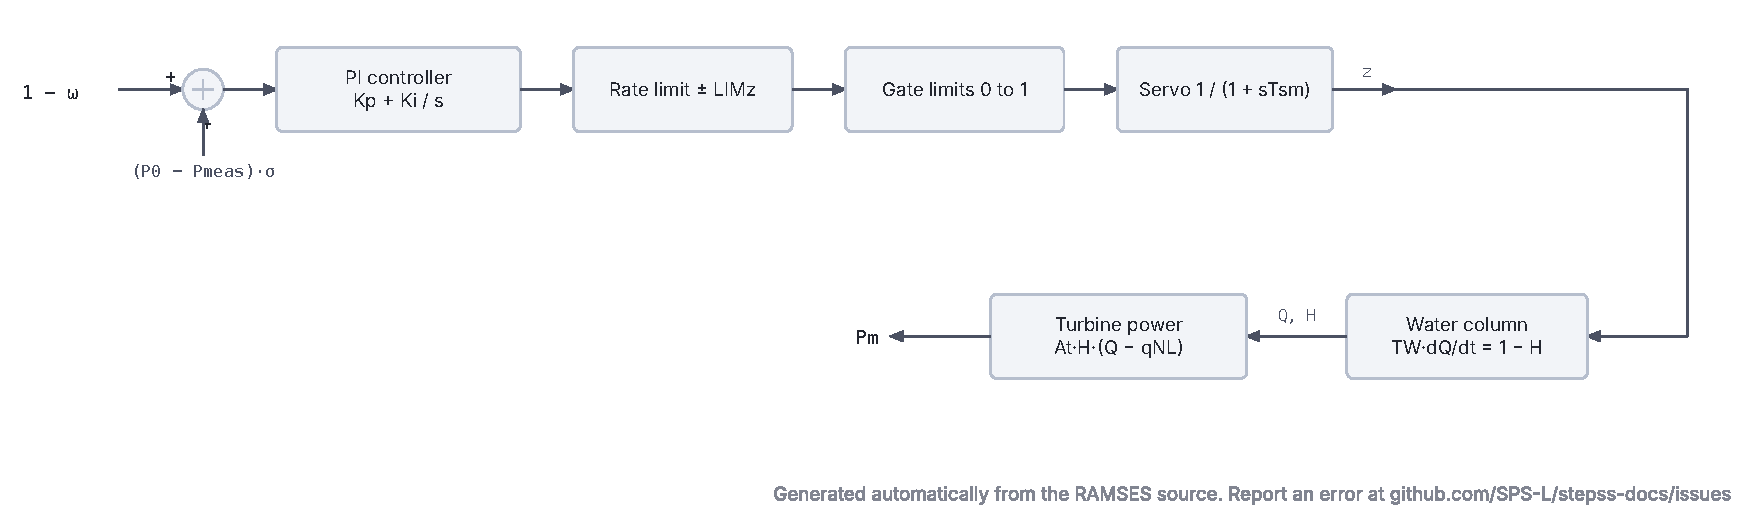
\includegraphics[width=0.98\linewidth]{figures/tor-hydro-generic1-light}
\caption{HYDRO\_GENERIC1 block diagram.}
\end{figure}

\subsection{Usage Example}\label{model-tor-custom:usage-example-3}

\textbf{RAMSES Data File}

\begin{Verbatim}
SYNC_MACH g1  g1  1. 1.  0.  0.   800. 760. 3. 0. 0.95
                    XT   0.15  1.1  0.25   0.2   0.7   *   0.2  0.1  6.0257  0.  5.00  0.05  *  0.1
              EXC GENERIC1   1.8991 -0.1  0.  1.  100. -1. -11  10.  70.  10.  20. 0.1  0.  4.
                                1     75.   15.    0.2    0.01     0.2    0.01    -0.1    0.1
              TOR HYDRO_GENERIC1  0.04  2.0  0.  2.00  0.40  0.2  0.1  1.0 ;
              !                   SIGMA  TP  Qv   KP    KI   TSM LIMZDOT TW
\end{Verbatim}

\textbf{Notes}

\begin{itemize}
\tightlist
\item
  \texttt{TW} (water-starting time) is the most influential parameter; typical values are 0.5--3 s.
\item
  Increase \texttt{KP} / \texttt{KI} carefully: large values can cause governor instability with high \texttt{TW}.
\item
  \texttt{Qv\ =\ 0} assumes no no-load losses.
\item
  Parameters follow the order in \texttt{dyn\_A.txt}: \texttt{SIGMA\ TP\ Qv\ KP\ KI\ TSM\ LIMZDOT\ TW}.
\end{itemize}

\begin{center}\rule{0.5\linewidth}{0.5pt}\end{center}

\section{\texorpdfstring{HYDRO\_DG (\texttt{tor\_HYDRO\_DG})}{HYDRO\_DG (tor\_HYDRO\_DG)}}\label{model-tor-custom:hydro_dg-tor_hydro_dg}

The data-file model name is \texttt{HYDRO\_DG}. Registered since 3.76.

\subsection{Scientific Description}\label{model-tor-custom:scientific-description-4}

A hydraulic turbine governor for a \textbf{dispersed generation unit that holds an active-power
setpoint and does not provide primary frequency response}.

The penstock and turbine are exactly those of \hyperref[model-tor-custom:hydro_generic1-tor_hydro_generic1]{\texttt{HYDRO\_GENERIC1}}.
What differs is the governor control law, and the difference is the point of the model.
\texttt{HYDRO\_GENERIC1} is a \textbf{speed governor}: its error signal carries an unconditional frequency
term, so the unit responds to system frequency whether or not that is wanted. \texttt{HYDRO\_DG}
regulates power alone.

\textbf{PI power regulator:}

The error is the deviation from the setpoint captured at initialisation, with no droop term
and no speed term:

\[
e = P^{*} - P
\]

\[
\dot{x}_{I} = K_i \cdot e, \qquad z_{demand} = K_p \cdot e + x_{I}
\]

There is no measurement lag on \(P\), so the regulator acts on the instantaneous electrical
power. The gate follows through a servo of time constant \(T_{sm}\), rate-limited to
\(\pm LIM_{\dot{z}}\) and position-limited to \([0, 1]\).

\textbf{Water column and turbine}, identical to \texttt{HYDRO\_GENERIC1}:

\[
T_W \cdot \frac{dQ}{dt} = 1 - H, \qquad H = \left(\frac{Q}{z}\right)^{2}
\]

\[
T_m \cdot \omega = \frac{(Q - Q_v) \, H}{1 - Q_v}
\]

\textbf{Parameters:}

\begin{small}\begin{longtable}[]{@{}lll@{}}
\toprule\noalign{}
Parameter & Index & Description \\
\midrule\noalign{}
\endhead
\bottomrule\noalign{}
\endlastfoot
\texttt{Qv} & 1 & No-load water flow fraction (pu) \\
\texttt{Kp} & 2 & PI proportional gain \\
\texttt{Ki} & 3 & PI integral gain \\
\texttt{TSM} & 4 & Gate servo time constant (s) \\
\texttt{LIMZDOT} & 5 & Gate velocity limit (pu/s) \\
\texttt{TW} & 6 & Water starting time (s) \\
\end{longtable}\end{small}

These are exactly parameters 3 to 8 of \texttt{HYDRO\_GENERIC1}, in the same order. \texttt{HYDRO\_GENERIC1}
precedes them with \texttt{SIGMA} (droop) and \texttt{Tmes} (speed measurement lag), and those two are what
\texttt{HYDRO\_DG} does not have. Setting \texttt{SIGMA} to zero in \texttt{HYDRO\_GENERIC1} does \textbf{not} reproduce
\texttt{HYDRO\_DG}, because the frequency term survives.

\textbf{Implementation details:}
- \texttt{nbxvar\ =\ 5}, \texttt{nbzvar\ =\ 2}, \texttt{nbdata\ =\ 6}, \texttt{nbaddpar\ =\ 1}
- Additional: \texttt{prm(7)\ =\ Pset}, the initial electrical power, captured at initialisation
- Observables: \texttt{z}, \texttt{Q}, \texttt{H}, \texttt{Pm}, \texttt{Pset}

\begin{figure}[htbp]
\centering
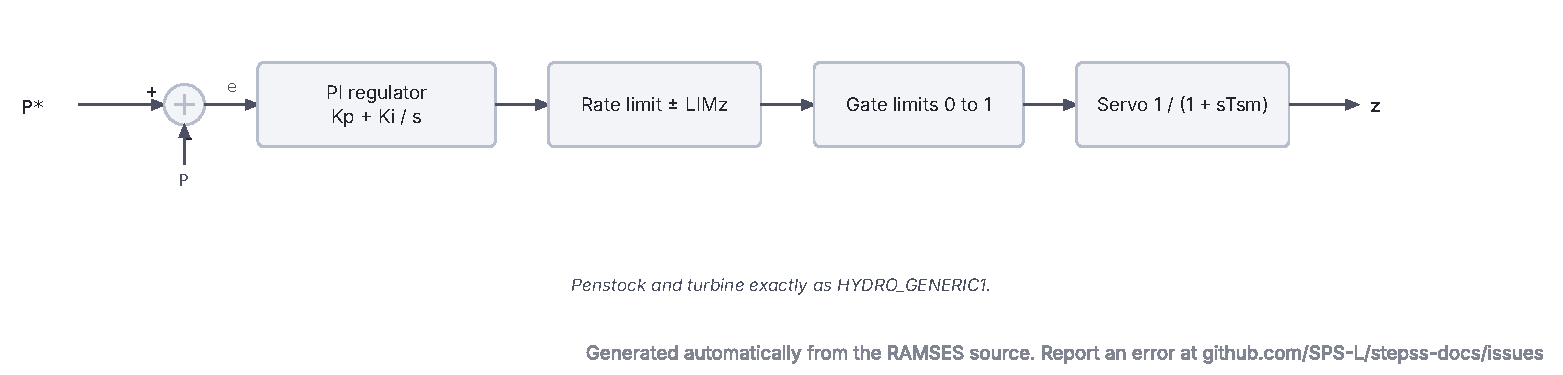
\includegraphics[width=0.98\linewidth]{figures/tor-hydro-dg-light}
\caption{HYDRO\_DG block diagram.}
\end{figure}

\subsection{Usage Example}\label{model-tor-custom:usage-example-4}

\textbf{RAMSES Data File}

\begin{Verbatim}
SYNC_MACH G4  N4 1. 1.  0.  0. 5 4.5 3. 0. 1.9333
              XT  0.0937  2.027  0.210  0.173  2.027  *  0.173  0.1  6  0.00  3.1  0.0387  *  0.0387
              EXC AVR_DG  2.865 -0.1  0.  1.  100. -1. -20  10  50  4  20  0.1  0  5
                          1  0.  5.  1.  1.  1.  1.  0.  0.
                          0.04  0.06  -0.2  0.33
              TOR HYDRO_DG  0.0  0.1  0.4  0.2  0.1  1.0 ;
              !             Qv   Kp   Ki   TSM LIMZDOT TW
\end{Verbatim}

\textbf{Notes}

\begin{itemize}
\tightlist
\item
  The setpoint is \textbf{not} a parameter. \texttt{Pset} is captured from the power-flow solution at
  initialisation, so the unit holds whatever it was dispatched to.
\item
  Because there is no frequency term, a system built only of these units has no primary
  frequency control. That is deliberate for dispersed generation studies, and it is worth
  being explicit about when interpreting a frequency response.
\item
  \texttt{Qv\ =\ 0} assumes no no-load losses.
\item
  The head relation divides by the gate position, which is floored at 1e-3 in the
  implementation so a fully closed gate cannot produce a division by zero.
\end{itemize}

\begin{center}\rule{0.5\linewidth}{0.5pt}\end{center}

\section{tor\_gasturbm}\label{model-tor-custom:tor_gasturbm}

\begin{docsnote}{Note}

Callable since 3.79. Earlier releases compiled this model under no name, so a data file referring to it was rejected.

\end{docsnote}

\subsection{Scientific Description}\label{model-tor-custom:scientific-description-5}

The \texttt{tor\_gasturbm} model is a \textbf{gas turbine} governor following a multi-stage combustion model. It captures the compressor, fuel system, combustion chamber delay, and turbine torque characteristic. The name suffix \texttt{m} indicates a modified version.

\textbf{Speed governor:}

The governor error drives a PI controller producing a fuel demand signal. The speed governor uses:

\[
e_{gov} = (\omega_{ref} - \omega) / TDSP - STAT \cdot P_{elec}
\]

with saturation limits \([MIN,\, MAX]\).

\textbf{Fuel system and combustion:}

The fuel valve position \texttt{g1} is driven through:
- A speed governor with gain \(ZZ\) and lead--lag time constants determined by \(XX\), \(YY\)
- A fuel flow path through first-order lag \(TVALVE\)
- Combustion chamber lag \(TGAZ\)

\textbf{Turbine output:}

The turbine mechanical power follows:

\[
P_m = BF2 \cdot g_{comb} + AF2
\]

where \(g_{comb}\) is the combustion output through lag \(TCD\).

Additional thermodynamic correction terms involve \(TF\) (flame lag) and \(ECR\) (exhaust correction ratio).

\textbf{Parameters from Fortran source (prm array):}

\begin{small}\begin{longtable}[]{@{}lll@{}}
\toprule\noalign{}
Index & Name & Description \\
\midrule\noalign{}
\endhead
\bottomrule\noalign{}
\endlastfoot
1 & \texttt{TDSP} & Speed droop time constant (s) \\
2 & \texttt{STAT} & Steady-state gain \\
3 & \texttt{ZZ} & Governor proportional gain \\
4 & \texttt{XX} & Lead numerator factor \\
5 & \texttt{YY} & Lag denominator factor \\
6 & \texttt{SACC} & Acceleration constant \\
7 & \texttt{MIN} & Minimum fuel valve position (pu) \\
8 & \texttt{MAX} & Maximum fuel valve position (pu) \\
9 & \texttt{TVALVE} & Fuel valve time constant (s) \\
10 & \texttt{TGAZ} & Combustion chamber time constant (s) \\
11 & \texttt{TF} & Flame lag time constant (s) \\
12 & \texttt{ECR} & Exhaust correction ratio \\
13 & \texttt{TCD} & Compressor discharge time constant (s) \\
14 & \texttt{BF2} & Turbine power output slope \\
15 & \texttt{AF2} & Turbine power output intercept (pu) \\
\end{longtable}\end{small}

\textbf{Implementation details:}
- \texttt{nbxvar\ =\ 10}, \texttt{nbzvar\ =\ 4}, \texttt{nbdata\ =\ 15}, \texttt{nbaddpar\ =\ 1}
- Additional: \texttt{prm(16)\ =\ SETPOINT} (initialised from load-flow power)
- Observables: \texttt{g2}, \texttt{x4}, \texttt{g1}

\subsection{Usage Example}\label{model-tor-custom:usage-example-5}

\textbf{RAMSES Data File}

\begin{Verbatim}
SYNC_MACH g1  g1  1. 1.  0.  0.   800. 760. 3. 0. 0.95
                    XT   0.15  1.1  0.25   0.2   0.7   *   0.2  0.1  6.0257  0.  5.00  0.05  *  0.1
              EXC GENERIC1   1.8991 -0.1  0.  1.  100. -1. -11  10.  70.  10.  20. 0.1  0.  4.
                                1     75.   15.    0.2    0.01     0.2    0.01    -0.1    0.1
              TOR GASTURBM  0.05  1.0  25.0  0.50  1.0  1.0  0.0  1.0  0.05  0.40  0.01  0.0  0.20  1.0  0.0 ;
              !              TDSP STAT  ZZ    XX   YY  SACC MIN  MAX TVALVE TGAZ   TF   ECR   TCD  BF2  AF2
\end{Verbatim}

\begin{center}\rule{0.5\linewidth}{0.5pt}\end{center}

\section{tor\_govclasm}\label{model-tor-custom:tor_govclasm}

\begin{docsnote}{Note}

Callable since 3.79. Earlier releases compiled this model under no name, so a data file referring to it was rejected.

\end{docsnote}

\subsection{Scientific Description}\label{model-tor-custom:scientific-description-6}

The \texttt{tor\_govclasm} model is a \textbf{classical thermal governor} with a composite control law including deadband, droop, integral control, and combustion dynamics. The name stands for ``governor classical model''.

\textbf{Speed governor with deadband and droop:}

The speed error passes through a deadband \([DBON, DEADB]\) before entering a proportional--integral controller. The integral path has saturation at \(MAXINT\) and gain \(ALPHA\). The reset time \(TRES\) determines the integration rate.

\textbf{Valve and combustion dynamics:}

The valve demand passes through:
1. A governor integrator with time constant \(TSM\), its rate held inside \([VFN,\, V0]\)
2. A first-order lag \(TFV\) (valve actuator)
3. A rate limiter \([PVARMIN,\, PVARMAX]\) (with gain \(GPVAR\)) representing fuel response
4. A combustion/steam chest lag \(KCR\), \(TCR\) producing fuel flow
5. Lower bound: \(MINFUEL\)
6. Transport delay \(TDELAY\) (approximated)
7. Turbine output through lag \(TCH\) with limits \([PMIN,\, PMAX]\)

\textbf{Parameters from Fortran source (prm array):}

\begin{small}\begin{longtable}[]{@{}
  >{\raggedright\arraybackslash}p{(\linewidth - 6\tabcolsep) * \real{0.1465}}
  >{\raggedright\arraybackslash}p{(\linewidth - 6\tabcolsep) * \real{0.2305}}
  >{\raggedright\arraybackslash}p{(\linewidth - 6\tabcolsep) * \real{0.6230}}
@{}}
\toprule\noalign{}
\begin{minipage}[b]{\linewidth}\raggedright
Index
\end{minipage} & \begin{minipage}[b]{\linewidth}\raggedright
Name
\end{minipage} & \begin{minipage}[b]{\linewidth}\raggedright
Description
\end{minipage} \\
\midrule\noalign{}
\endhead
\bottomrule\noalign{}
\endlastfoot
1 & \texttt{STAT} & Governor static characteristic selector \\
2 & \texttt{DEADB} & Deadband half-width (pu) \\
3 & \texttt{DBON} & Deadband onset (pu) \\
4 & \texttt{TSM} & Speed measurement / filter time constant (s) \\
5 & \texttt{V0} & Maximum valve opening rate, upper limit on the governor integrator rate (pu/s) \\
6 & \texttt{VFN} & Minimum valve rate, applied directly as the lower bound, so normally negative (pu/s) \\
7 & \texttt{TFV} & Valve actuator time constant (s) \\
8 & \texttt{VFR} & Fuel flow rate limit (pu/s) \\
9 & \texttt{MAXINT} & Maximum integral output (pu) \\
10 & \texttt{ALPHA} & Integral controller gain \\
11 & \texttt{TRES} & Integral reset time (s) \\
12 & \texttt{GOMP} & Governor proportional gain \\
13 & \texttt{PVARMAX} & Maximum power variation rate (pu) \\
14 & \texttt{PVARMIN} & Minimum power variation rate (pu) \\
15 & \texttt{GPVAR} & Power variation gain \\
16 & \texttt{KCR} & Combustion gain \\
17 & \texttt{TCR} & Combustion time constant (s) \\
18 & \texttt{MINFUEL} & Minimum fuel flow (pu) \\
19 & \texttt{TDELAY} & Combustion transport delay (s) \\
20 & \texttt{PMAX} & Maximum turbine output (pu) \\
21 & \texttt{TCH} & Steam chest / turbine lag (s) \\
22 & \texttt{PMIN} & Minimum turbine output (pu) \\
\end{longtable}\end{small}

\textbf{Implementation details:}
- \texttt{nbxvar\ =\ 6}, \texttt{nbzvar\ =\ 10}, \texttt{nbdata\ =\ 22}, \texttt{nbaddpar\ =\ 1}
- Additional: \texttt{prm(23)\ =\ P0} (initialised from load-flow power)
- Observables: \texttt{x2}, \texttt{b3}, \texttt{b4}

\subsection{Usage Example}\label{model-tor-custom:usage-example-6}

\textbf{RAMSES Data File}

\begin{Verbatim}
SYNC_MACH g1  g1  1. 1.  0.  0.   800. 760. 3. 0. 0.95
                    XT   0.15  1.1  0.25   0.2   0.7   *   0.2  0.1  6.0257  0.  5.00  0.05  *  0.1
              EXC GENERIC1   1.8991 -0.1  0.  1.  100. -1. -11  10.  70.  10.  20. 0.1  0.  4.
                                1     75.   15.    0.2    0.01     0.2    0.01    -0.1    0.1
              TOR GOVCLASM  1.0  0.003  0.001  0.10  1.0  1.0  0.30  0.5  1.0  1.0  5.0  25.0  0.10  -0.10  0.05  1.0  0.20  0.05  0.30  1.05  0.30  0.05 ;
              !              STAT DEADB  DBON   TSM   V0  VFN   TFV  VFR MAXINT ALPHA TRES  GOMP PVARMAX PVARMIN GPVAR KCR  TCR MINFUEL TDELAY PMAX  TCH  PMIN
\end{Verbatim}

\begin{center}\rule{0.5\linewidth}{0.5pt}\end{center}

\section{tor\_govhydr}\label{model-tor-custom:tor_govhydr}

\begin{docsnote}{Note}

Callable since 3.79. Earlier releases compiled this model under no name, so a data file referring to it was rejected.

\end{docsnote}

\subsection{Scientific Description}\label{model-tor-custom:scientific-description-7}

The \texttt{tor\_govhydr} model is a \textbf{simplified hydraulic governor} with PI control and a non-linear penstock. It differs from \texttt{tor\_hydro\_generic1} in its simplified turbine characteristic and simpler water-column formulation.

\textbf{PI governor:}

\[
\dot{x}_2 = K_I \cdot e, \quad x_2 \in [0, 1]
\]

\[
z_{demand} = K_P \cdot e + x_2
\]

where the speed error \(e = P_0/\omega - T_m - \omega \cdot STAT + \ldots\) accounts for the droop and steady-state bias.

\textbf{Penstock (two-lag water column):}

\[
T_{CE1} \cdot \frac{dx_3}{dt} = P - x_3(1 + T_{CE2}/T_{CE1})
\]

The turbine mechanical power is computed via an empirical quadratic:

\[
P_m = 1.35 \cdot z - 0.7 z^2
\]

derived from the non-linear head-flow curve approximated at initialisation.

\textbf{Parameters from Fortran source:}

\begin{small}\begin{longtable}[]{@{}
  >{\raggedright\arraybackslash}p{(\linewidth - 6\tabcolsep) * \real{0.1393}}
  >{\raggedright\arraybackslash}p{(\linewidth - 6\tabcolsep) * \real{0.1926}}
  >{\raggedright\arraybackslash}p{(\linewidth - 6\tabcolsep) * \real{0.6681}}
@{}}
\toprule\noalign{}
\begin{minipage}[b]{\linewidth}\raggedright
Index
\end{minipage} & \begin{minipage}[b]{\linewidth}\raggedright
Name
\end{minipage} & \begin{minipage}[b]{\linewidth}\raggedright
Description
\end{minipage} \\
\midrule\noalign{}
\endhead
\bottomrule\noalign{}
\endlastfoot
1 & \texttt{STAT} & Steady-state gain selector \\
2 & \texttt{KP} & Proportional gain \\
3 & \texttt{KI} & Integral gain \\
4 & \texttt{TC} & Governor/servo time constant (s) \\
5 & \texttt{V0} & Maximum gate opening rate, upper limit on gate velocity (pu/s) \\
6 & \texttt{VF} & Maximum gate closing rate, entered as a positive magnitude and applied as \(-V_F\) (pu/s) \\
7 & \texttt{TCE2} & Second penstock time constant (s) \\
8 & \texttt{TCE1} & First penstock time constant (s) \\
\end{longtable}\end{small}

\textbf{Implementation details:}
- \texttt{nbxvar\ =\ 4}, \texttt{nbzvar\ =\ 4}, \texttt{nbdata\ =\ 8}, \texttt{nbaddpar\ =\ 1}
- Additional: \texttt{prm(9)\ =\ P0} (initialised from load-flow power)
- No observables defined (\texttt{nbobs\ =\ 0})

\subsection{Usage Example}\label{model-tor-custom:usage-example-7}

\textbf{RAMSES Data File}

\begin{Verbatim}
SYNC_MACH g1  g1  1. 1.  0.  0.   800. 760. 3. 0. 0.95
                    XT   0.15  1.1  0.25   0.2   0.7   *   0.2  0.1  6.0257  0.  5.00  0.05  *  0.1
              EXC GENERIC1   1.8991 -0.1  0.  1.  100. -1. -11  10.  70.  10.  20. 0.1  0.  4.
                                1     75.   15.    0.2    0.01     0.2    0.01    -0.1    0.1
              TOR GOVHYDR  1.0  2.0  0.5  0.10  1.0  1.0  1.0  5.0 ;
              !             STAT  KP   KI   TC   V0   VF  TCE2 TCE1
\end{Verbatim}

\textbf{Notes}

\begin{itemize}
\tightlist
\item
  \texttt{TCE1} corresponds roughly to the water-starting time \(T_W\).
\item
  \texttt{TCE2/TCE1} sets the ratio of the two penstock lags.
\end{itemize}

\begin{center}\rule{0.5\linewidth}{0.5pt}\end{center}

\section{tor\_govnuc}\label{model-tor-custom:tor_govnuc}

\begin{docsnote}{Note}

Callable since 3.79. Earlier releases compiled this model under no name, so a data file referring to it was rejected.

\end{docsnote}

\subsection{Scientific Description}\label{model-tor-custom:scientific-description-8}

The \texttt{tor\_govnuc} model is a \textbf{nuclear plant governor} with deadband, droop, integral control, and a non-linear turbine characteristic via \texttt{GOMP} (the gain of the output multiplier). It is structurally similar to \texttt{tor\_govclasm} but tailored for the slower, tightly-regulated dynamics of nuclear steam supply systems.

\textbf{Speed governor:}

The speed error passes through a deadband \([DBON, DEADB]\):

\[
e = \text{deadband}(\omega_{ref} - \omega) - STAT \cdot (P - P_0)
\]

The error enters an integrator with rate limits \([GRADMIN, GRADMAX]\) (pu/s) filtered through a ramp time \(TGRAD\). The integrator output \(x_I\) passes through a servo \(TSM\).

\textbf{Turbine characteristic with GOMP:}

The turbine output is non-linearly mapped through a gain \(GOMP\):

\[
P_m = \min\!\left(\frac{x_I}{GOMP},\, 1\right) \cdot f(x_I)
\]

where the limiter prevents over-power and \(f\) is a piecewise-linear characteristic.

The steam-valve rate is held inside \([VFN,\, V0]\), then passes the valve actuator lag \(TFV\), the reset lag \(TRES\) and \(GOMP\) to produce the final torque. \(VFR\) overrides the rate during fast valving, a path the shipped model never takes: the code fixes its selector at 1 and leaves the fast-valving logic unwritten.

\textbf{Parameters from Fortran source:}

\begin{small}\begin{longtable}[]{@{}
  >{\raggedright\arraybackslash}p{(\linewidth - 6\tabcolsep) * \real{0.1410}}
  >{\raggedright\arraybackslash}p{(\linewidth - 6\tabcolsep) * \real{0.2284}}
  >{\raggedright\arraybackslash}p{(\linewidth - 6\tabcolsep) * \real{0.6306}}
@{}}
\toprule\noalign{}
\begin{minipage}[b]{\linewidth}\raggedright
Index
\end{minipage} & \begin{minipage}[b]{\linewidth}\raggedright
Name
\end{minipage} & \begin{minipage}[b]{\linewidth}\raggedright
Description
\end{minipage} \\
\midrule\noalign{}
\endhead
\bottomrule\noalign{}
\endlastfoot
1 & \texttt{STAT} & Governor static characteristic selector \\
2 & \texttt{DEADB} & Deadband half-width (pu) \\
3 & \texttt{DBON} & Deadband onset (pu) \\
4 & \texttt{GRADMAX} & Maximum load gradient (pu/s) \\
5 & \texttt{GRADMIN} & Minimum load gradient / unloading rate (pu/s) \\
6 & \texttt{TGRAD} & Ramp filter time constant (s) \\
7 & \texttt{TSM} & Servo time constant (s) \\
8 & \texttt{V0} & Maximum valve opening rate, upper limit on the steam-valve rate (pu/s) \\
9 & \texttt{VFN} & Minimum valve rate, applied directly as the lower bound, so normally negative (pu/s) \\
10 & \texttt{TFV} & Valve actuator time constant (s) \\
11 & \texttt{VFR} & Valve rate limit (pu/s) \\
12 & \texttt{ALPHA} & Integral gain \\
13 & \texttt{TRES} & Reset time constant (s) \\
14 & \texttt{GOMP} & Output power gain \\
\end{longtable}\end{small}

\textbf{Implementation details:}
- \texttt{nbxvar\ =\ 4}, \texttt{nbzvar\ =\ 8}, \texttt{nbdata\ =\ 14}, \texttt{nbaddpar\ =\ 1}
- Additional: \texttt{prm(15)\ =\ P0} (initialised from load-flow power)
- Observable: \texttt{TM}

\subsection{Usage Example}\label{model-tor-custom:usage-example-8}

\textbf{RAMSES Data File}

\begin{Verbatim}
SYNC_MACH g1  g1  1. 1.  0.  0.   800. 760. 3. 0. 0.95
                    XT   0.15  1.1  0.25   0.2   0.7   *   0.2  0.1  6.0257  0.  5.00  0.05  *  0.1
              EXC GENERIC1   1.8991 -0.1  0.  1.  100. -1. -11  10.  70.  10.  20. 0.1  0.  4.
                                1     75.   15.    0.2    0.01     0.2    0.01    -0.1    0.1
              TOR GOVNUC  1.0  0.005  0.002  0.02  -0.02  10.0  5.0  1.0  1.0  0.50  0.10  1.0  20.0  1.0 ;
              !            STAT DEADB   DBON GRADMAX GRADMIN TGRAD TSM  V0  VFN   TFV   VFR ALPHA  TRES  GOMP
\end{Verbatim}

\textbf{Notes}

\begin{itemize}
\tightlist
\item
  Nuclear plants typically have slow load-following characteristics: \texttt{GRADMAX} is typically 0.005--0.02 pu/s.
\item
  The \texttt{DEADB} is important to prevent hunting around the setpoint.
\item
  \texttt{GOMP} scales the turbine output; set to 1.0 for standard normalisation.
\end{itemize}
